% specifies the documnt class. We usually use article but there are others. 
\documentclass{article}              

% these are standard packages used for the math symbols
\usepackage{amsmath,amssymb,amsthm, enumitem, hyperref, tabto} 
\usepackage[T1]{fontenc}
\usepackage[utf8]{inputenc}
\usepackage[english]{babel}
\usepackage{fancyhdr}
\usepackage{lastpage}
\usepackage{colortbl}
\usepackage[pdftex]{graphicx}
\usepackage{float}
\graphicspath{ {./Photos/} }

\definecolor{aqua}{rgb}{0.0, 1.0, 1.0}
\definecolor{orange}{rgb}{1.0, 0.65, 0.0}

% These commands below is to make sure the numbering of these are consistent with theorem
% If you are not sure what something means, delete them, build a new file and see the
% difference between the files. You can ignore this part for now.
\newtheorem{theorem}{Theorem}[section]
\newtheorem{conjecture}[theorem]{Conjecture}
\newtheorem{observation}[theorem]{Observation}
\newtheorem{definition}[theorem]{Definition}
\newtheorem{corollary}[theorem]{Corollary}
\newtheorem{lemma}[theorem]{Lemma}
\newtheorem{example}[theorem]{Example}
\newtheorem{remark}[theorem]{Remark}
\newtheorem{notation}[theorem]{Notation}

% Title of your project
\title{%
  \Huge Ramanujan's Square \\
  \LARGE Detailed Analysis\\
  \Large A DV2136 Project}

% The author command places text right after title
\author{by \\
\Large Afzal (h1810003) \\
\Large Prannaya Gupta (h1810124) \\
\Large Yap Yuan Xi (h1810166) \\
}

\date{\Large July - September 2019}

\begin{document}

\maketitle

\tableofcontents
\newpage
\section{An Introduction}

\subsection{Inspiration}
We are working on Ramanujan's Magic Squares because it is a fascinating phenomenon. It is created using the date of the creator. Its an interesting concept and we really want to build upon it. We want to extend on this concept so we can see what may behold. We want to try. And we want to see if this paper bears any fruit at all.

\newpage
\subsection{Magic Squares}

\subsubsection{Abstract}
In real life situations, some problems relating to division of objects equal in numbers and value can be easily solved by constructing a semi magic square or a magic square in accordance with the given conditions. Mathematics is magic if we can either use one formula for a wide range of applications or the formula itself will produce magic properties.

\subsubsection{A Brief History of the Magic Square}
Magic squares were known to Chinese mathematicians, and Arab mathematicians, possibly as early as the $7^{th}$ century, when the Arabs conquered northwestern parts of the Indian subcontinent and to learned Indian mathematicians and astronomers, including other aspects of combinatorical mathematics. ‘Cornelius Agrippa’ (1486 B.C. to 1535 B.C.) of China is believed to be the first for construction of magic squares.

\subsubsection{The Properties of a general Magic Square}
A general Magic Square is the arrangement of random number within the cell such that sum of each row = each column = each diagonal. The common sum is known as ‘Magic Constant’ or ‘Magic Number’. If the above condition is valid only for the sum of elements of rows and columns and not for the diagonal elements, then that array is known as a semi magic square. All magic squares are semi magic squares. A normal magic square contains the integers from 1 to $n^2$. The constant sum in every row, column and diagonal is called the magic constant or magic sum, S. The magic constant of a normal magic square with continuous numbers depends only on n and has the value $S = \frac{n(n^2+1)}{2}$

\subsection{Variants of Magic Squares}
\begin{center}
    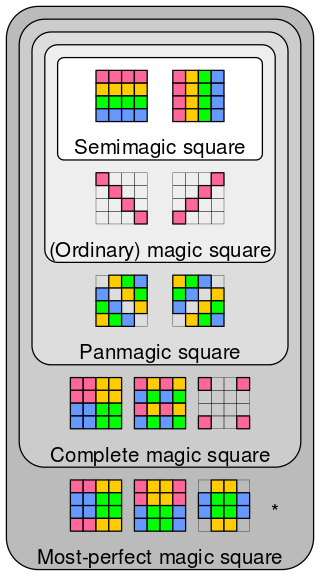
\includegraphics[width=0.3\textwidth]{Photos/MagicSquareHeirarchy.png}
\end{center}
\subsubsection{Semimagic Squares}
    In semimagic squares, the sums of the rows and columns add up to the same number.
\subsubsection{(Ordinary) Magic Squares}
    In ordinary magic squares, the sum of the rows, columns and the diagonals adds up to the same number.
\subsubsection{Panmagic Squares}
    In panmagic squares, the sum of the rows, columns, the diagonals and broken diagonals add up to the same number
\subsubsection{Complete Magic Squares}
    In complete magic squares, the corners, boxes and alternating rows and columns add up to the same sum as well.
\subsubsection{Most Perfect Squares}
    An example of the perfect magic square is the Ramanujan's Square, but including the sums of alternating rows and columns.

\subsection{The Area of Our Investigation}
We are trying to investigate The Ramanujan's Magic Square, a magic square devised by the genius mathematician Srinivasa Ramanujan which has a number of exciting properties.

\newpage
\section{Srinivasa Ramanujan, the creator}
\tab Born in 1887, Ramanujan was a young Indian student.
By the age of 23 Ramanujan was making important new discoveries in mathematics. Professor G.H. Hardy recognised a touch of pure genius in Ramanujan’s theorems. Hardy recognised his talents and arranged to bring Ramanujan to England. Ramanujan decided to accept Hardy’s offer, and on 17 March, 1914 he set out by ship to England.
\subsection{England}
In Cambridge, the young Indian set about working on hundreds of new theorems. Hardy said: “I have never met Ramanujan’s equal.”\cite{studyMagicSquare} However, Ramanujan did not fare so well in his private life. His fragile health suffered. He even became suicidal.
Sadly, Ramanujan never regained his health. He died on 20 April, 1920 in a care home near Madras (now Chennai). He continued working on new theorems even on his death bed. Showing his true Mathematical spirit.\cite{historyRamanujan}

\newpage
\section{Primary Basis of our Investigation}

\subsection{Ramanujan's Magic Square}
\tab We are investigating Srinivasa Ramanujan's Magic Square. It is noticed that in a normal magic square the columns and rows give the same sum. However in this Magic Square, there are other ways to get the same sum. Like the corners, the diagonals and many more.

\subsubsection{What we can derive from the square}
\tab This is very intriguing to us for its adaptability to any birthday date, and made us want to find out how it works and how this is possible. We want to explore the magic of this mathematical square.

\newpage
\section{How does it work?}

\subsection{Description}
\tab This square has a huge number of possible magic square possibilities. You can consider a huge amount magic square patterns like 'By Row', 'By Column', 'By Quarter'.  Below is a definitive list:

\begin{itemize}
  \item The sum of any column is a number y
  \item The sum of any row is the number y
  \item The sum of any diagonal is the number y
  \item The sum of any 2x2 is the number y (except for those in the middle two columns)
\end{itemize}

However, the real miracle of this square its ability to seemingly morph from one's birthday. The main magic square used as an example is actually derived from Ramanujan's birth date, 22 December 1887, thus amounting the sum y as 139. This is an interesting graphic and provides a majorly interesting phenomenon.

\subsection{Graphical Representation}
\begin{figure}[H]
\begin{center}
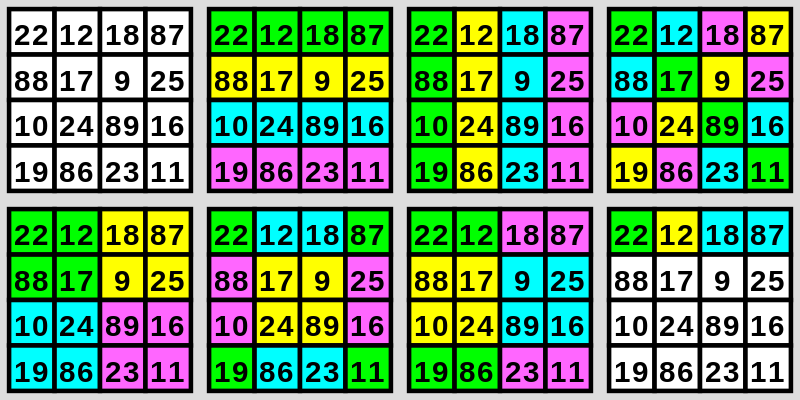
\includegraphics[scale = 0.4]{MagicSquare} 
\cite{magicSquare}
\caption{These diagrams show the ways in which the numbers of the Square add up to 139 in the main Ramanujan Square}
\end{center}
\end{figure}

\newpage
\subsection{The Solution}
\begin{figure}[H]
\begin{center}
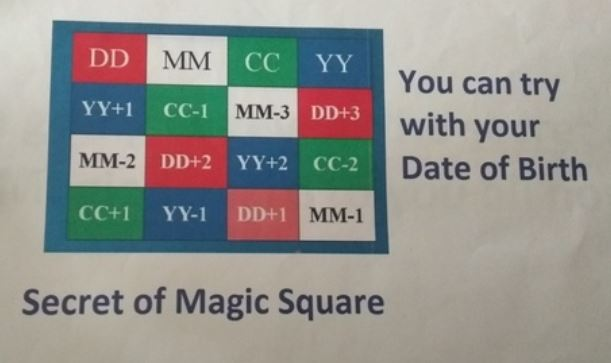
\includegraphics[scale = 1.0]{RamanujanSquare}
\cite{ramanujanSquare}
\caption{This diagram shows the algorithm by which the numbers of the Square add up to 139 in the main Ramanujan Square}
\end{center}
\end{figure}

\paragraph{
Let Me Explain: Consider the first row being the derivation.
}
\begin{equation*}
Sum_{given} = DD + MM + CC + YY
\end{equation*}
where DD is the date, MM is the month, CC is the century and YY is the year.

\paragraph{Now consider the first column.}
\begin{equation*}
Sum_{col_1} = DD + (MM-2) + (CC+1) + (YY+1) = DD + MM + CC + YY
\end{equation*}
\subparagraph{Therefore, $Sum_{col_1} = Sum_{given}$}

\paragraph{Try it yourself, this applies for every single property we showed, because the numbers are perfectly balanced.}

\newpage
\section{Extensions and Generalisations}

\subsection{Bigger Squares}
Can we make the square bigger.
    \subsubsection{5x5 Magic Square}
        Letting H, D, M, C, Y be the hour, the day, the month, the century and the year respectively. \\
        \def\arraystretch{2}
        \begin{center}
            \begin{tabular}{|c|c|c|c|c|}
                \hline
                 H + 0 & D + 0 & M + 0 & C + 0 & Y + 0  \\
                 \hline
                 D - 2 & C + 1 & Y + 1 & M + 3 & M - 3 \\
                 \hline
                 Y + 2 & M - 1 & D - 1 & H - 2 & C + 2 \\
                 \hline
                 M - 3 & H + 1 & C - 3 & Y + 2 & D + 3 \\
                 \hline
                 C + 3 & Y - 1 & H + 3 & D - 3 & M - 2 \\
                 \hline
            \end{tabular}\\
        \textbf{\\ Note: This magic square is only pandiagonal and has multiples of one of the numbers}
        \end{center}
    \subsubsection{6x6 Magic Square}
        Letting m, H, D, M, C and Y be the minute, the hour, the day, the month, the century and the year respectively. \\
        This table uses the minute of your birth, forming an even larger square. \\
        \def\arraystretch{2}
        \begin{center}
            \begin{tabular}{|c|c|c|c|c|c|}
                \hline
                 m + 0 & H + 0 & D + 0 & M + 0 & C + 0 & Y + 0  \\
                 \hline
                 M - 1 & Y + 1 & H - 3 & C + 3 & m - 2 & D + 2\\
                 \hline
                 D + 3 & m - 1 & C - 1 & H + 2 & Y - 2 & M - 1\\
                 \hline
                 Y + 2 & C - 4 & M - 3 & D + 1 & H + 3 & M + 1\\
                 \hline
                 H - 2 & D + 2 & m + 4 & Y - 2 & M - 1 & C - 1 \\
                 \hline
                 C - 2 & M + 2 & Y + 3 & m - 4 & D + 2 & H - 1 \\
                 \hline
            \end{tabular} \\
        \textbf{\\ Note: This is only a basic magic square with multiple repeated entries}
        \end{center}
        
\subsection{Other Forms}
Are there any other squares with the same properties?
There are many.\\
But first let us define some stuff.\\
We set D be Day, M be Month, C be century, Y be year. \\
For example, if your birthday was on 22 December 1887.\\ 
Then, D = 22, M = 12, C = 18, Y = 87.\\
    \subsubsection{Variation 1: Diagonal}
        \def\arraystretch{2}
        \begin{center}
            \begin{tabular}{|c|c|c|c|}
                \hline
                \cellcolor{yellow} D + 0 & Y + 2 & M - 1 & C - 1 \\
                \hline
                C - 2 & \cellcolor{green} M + 0 & Y - 1 & D + 3 \\
                \hline
                Y + 1 & D + 1 & \cellcolor{aqua} C + 0 & M - 2 \\
                \hline
                M + 1 & C - 3 & D + 2 & \cellcolor{orange} Y + 0 \\
                \hline
            \end{tabular}
        \end{center}
    \subsubsection{Variation 2: Box}
        \def\arraystretch{2}
        \begin{center}
            \begin{tabular}{|c|c|c|c|}
                \hline
                C - 2 & M + 1 & D + 2 & Y - 1 \\
                \hline
                Y + 1 & \cellcolor{yellow} D + 0 & \cellcolor{green} M + 0 & C - 1 \\
                \hline
                M - 1 & \cellcolor{aqua} C + 0 & \cellcolor{orange} Y + 0 & D + 1 \\
                \hline
                D + 2 & Y - 1 & C - 2 & M + 1 \\
                \hline
            \end{tabular}
        \end{center}
        
        
    \subsubsection{Variation 3: Column}
        \def\arraystretch{2}
        \begin{center}
            \begin{tabular}{|c|c|c|c|}
                \hline
                \cellcolor{yellow} D + 0 & C + 2 & Y - 1 & M - 1 \\
                \hline
                \cellcolor{green} M + 0 & Y - 2 & C - 1 & D + 3 \\
                \hline
                \cellcolor{aqua} C + 0 & D + 2 & M + 1 & Y - 3 \\
                \hline
                \cellcolor{orange} Y + 0 & M - 2 & D + 1 & C + 1 \\
                \hline
            \end{tabular}
        \end{center}
        
    \subsubsection{Method of making these squares}
        Looking at the above Variations. We believe that there is a method in the creation of these kinds of squares.
        
        This is the method we found while creating the squares
        
        \begin{enumerate}
            \item Set the beginning (Column, Row etc.) 
            \item Set each box to base of one of the four given variables 
            \item Set one number to differ
            \item Using that number set the others, keeping the beginning unchanged
            \item Check if it all add up and make changes if necessary. Repeat this till completion.
        \end{enumerate}
        
\subsection{Super Asymmetry}
Is there any form of derivation of the overall constant without any symmetrical significance?

Yes, yes there is.

\begin{center}
            \begin{tabular}{|c|c|c|c|}
                \hline
                \cellcolor{yellow} D + 0 & \cellcolor{yellow} M + 0 & \cellcolor{orange} C + 0 & \cellcolor{aqua} Y + 0 \\
                \hline
                \cellcolor{orange} Y + 1 & \cellcolor{aqua} C - 1 & \cellcolor{orange} M - 3 & \cellcolor{aqua} D + 3 \\
                \hline
                \cellcolor{aqua} M - 2 & \cellcolor{orange} D + 2 & \cellcolor{green} Y + 2 & \cellcolor{green} C - 2 \\
                \hline
                \cellcolor{green} D + 0 & \cellcolor{yellow} C + 2 & \cellcolor{yellow} Y - 1 & \cellcolor{green} M - 1 \\
                \hline
            \end{tabular}
        \end{center}

The sum of the numbers in the same coloured cell give the same sum.

\end{document}
